\documentclass[10pt]{article}

\input{/Users/gabesekeres/Dropbox/LaTeX_Docs/pset_preamble.tex}

\course{ECON 6200}
\pset{6}
\begin{document}
\maketitle

\textbf{\textit{n.b.}} Code is below, in the \href{code}{code section}. It is entirely in Julia

\begin{enumerate}
	\item \textbf{Bootstrap CI for the Median} \begin{enumerate} \item I drew 100 realizations from a standard normal distribution, fixing the seed for replicability. A histogram of my data is: \begin{figure}[H]\centering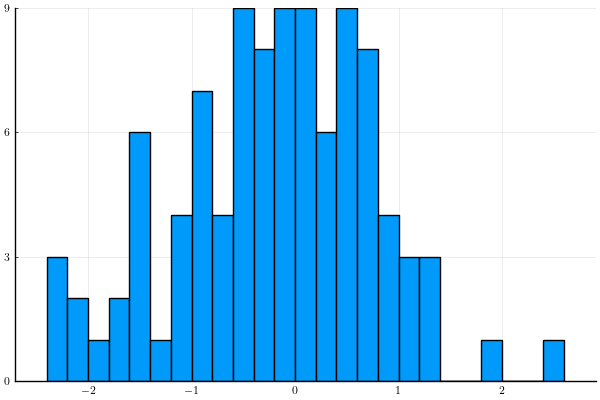
\includegraphics[width=10cm]{ps6_code/ps6_hist.png}\end{figure}The sample median is $-0.0899$, and the confidence intervals using the bootsrapped standard errors and percentiles are, respectively,\[(-0.3006,0.1207) \qquad ; \qquad (-0.3302,0.0871)\]Both cover zero, though they clearly reflect the skew of the original sample. \item I simulated this 1,000 times using different seeds, which took approximately 3.33 seconds to run. I got that the coverage of the standard error method was $0.889$, and the coverage of the percentile method was $0.895$. Interestingly, the average length of the percentile method was smaller at $0.405$ while the average length of the standard error method was $0.416$. \end{enumerate}
	\item \textbf{Bootstrap Failures} I first give the quick red flags for why bootstrapping may not work for the below cases: \begin{itemize}\item The Cauchy distribution has no finite moments, which raises an immediate red flag, since the sample mean does not have finite variance and does not converge to the population mean. The same is true for all moments. \item The red flag here is that there is a kink in the function at exactly the population mean. For bootstrapping, we want to find an interior minimum but there is no point where the derivative of $T_n$ is (only) zero in any open neighborhood of $\expect(X)$. \item When the true population mean is zero, we will have a large point mass at zero, and so the bootstrapped distribution will be degenerate, in a way that cannot be normalized by $\sqrt{n}$ \item Since $\max_i X_i < \alpha$ with probability 1, the order statistic is biased downwards in every finite sample. \end{itemize} I verified the final bootstrap failure using Julia, by simulating a resampling with sample size 100 on $U[0,1]$. I made a 95\% confidence interval for $\alpha$, and verified that the coverage probability over 1,000 repetitions was 0, since the bootstrap interval is always shorter than the real one and never reaches the true $\alpha = 1$. The code is below, and took 0.89 seconds to run. To get further intuition, observe that except in the event that 3 or more of the samples are exactly 1, the interval will always fail to include 1. The event that even one sample is equal to 1 has measure 0, and occurs with precisely probability 0. Included below is a histogram of the upper bound of the 1,000 intervals. \begin{figure}[H] \centering 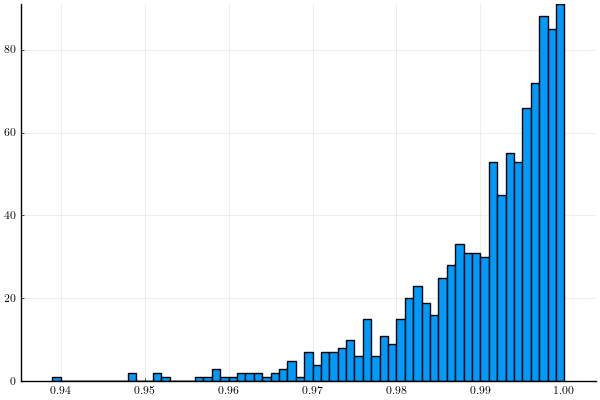
\includegraphics[width=10cm]{ps6_code/ps6_max.png}\end{figure}
\end{enumerate}





\newpage
\section*{Code}\label{code}

\lstinputlisting[language=Julia]{ps6_code/main.jl}

\end{document}